\chapter{The Simplified $P_N$ Equations}
\label{ch:spn_equations}

The neutron transport problem is complicated. Solutions cover a large
phase space and the problems of interest are often geometrically
complex, very large, or both, requiring tremendous computational
resources to generate an adequate solution. Modern deterministic
methods for large scale problems are commonly variants on the discrete
ordinates ($S_N$) method \citep{evans_denovo:_2010}. For full reactor
core neutronics simulations, the $S_N$ method requires potentially
trillions of unknown angular flux moments to be computed to achieve
good accuracy for the repsonses of interest
\citep{slaybaugh_acceleration_2011}. Other forms of the transport
problem, including the $P_N$ method, take on a simpler form than the
more common $S_N$ methods but lack in accuracy when compared while
still requiring considerable computational resources for solutions in
multiple dimensions.

In the 1960's, Gelbard developed an ad-hoc multidimensional extension
of the simple single dimension planar $P_N$ equations that created a
system of coupled, diffusion-like equations known as the simplified
$P_N$ ($SP_N$) equations. Up until around the 1990's, the $SP_N$
method was either widely unknown, widely unused, or combination of
both even though numerical studies showed promising results with
better solutions than diffusion theory and a significant reduction in
computational time over more accurate methods such as discrete
ordinates. Why did this happen? A significant problem, pointed out by
Larsen, was that little rigor had been applied to the formulation of
the $SP_N$ equations since their derivation through primarily
heuristic arguments. Instead, studies at that time focused on simply
comparing the results of the method to other contemporary transport
solution strategies. In addition, many problems of interest from the
literature at the time were either solved using nodal-type methods for
reactor-sized problems or $S_N$-type methods for benchmark problems
with intricate material configurations and potentially large flux
gradients over small spatial domains.

So why reconsider the $SP_N$ equations? Starting in the 1990's and
primarily due to Larsen and his colleagues, the $SP_N$ equations have
been given a more rigorous treatment with both variational and
asymptotic derivations performed as a means of verification. In
addition, these equations have been more rigorously studied as
solution methods to MOX fuel problems and have been shown to provide
accurate solutions. With this mathematical literature to provide a
solid numerical footing for the method, we look at its application to
today's challenge problems in full reactor core transport. The
reduction in numerical complexity of current full core deterministic
solution methods using the $S_N$ approximation could mean significant
savings in both compute time and memory required. In addition, the
characteristics of the solution to the transport problem for a steady
state reactor core permit diffusion theory to be used; a staple of the
nuclear industry since its inception. Therefore, if diffusion theory
is applicable, then finer grained solutions that capture more of the
physics contained in the transport equation should be possible with
the $SP_N$ method. In doing so, we also expect from the literature to
obtain computed responses on the order of accuracy we would expect
from an appropriately discretized $S_N$ method at a fraction of the
cost. 

To further motivate moving in this direction, recent developments in
the Exnihilo neutronics package at Oak Ridge National Laboratory have
permitted generation of the $SP_N$ system of equations for detailed
full core reactor models. By fully forming these equations and
formulating them as a linear algebra problem instead of using the
explicit iterative methods of the past, we now have access to all of
the modern advancements in computational linear algebra including
Krylov solvers for asymmetric systems and preconditioning methods such
as algebraic multigrid. This leads us to then explore the
applicability of our work in discrete Monte Carlo methods for linear
systems as a possible solution method for the $SP_N$ equations. If
formulated correctly, we hypothesize that signficant improvement in
usage of computational resources may be observed compared to modern
solution techniques such as those suggested due to the form of the
matrices generated by the discretization. In addition, solving the
$SP_N$ equations in this way also breaks away from the $S_N$ forms of
parallelism where spatial parallelism is achieved by an efficient
parallel sweep, angular efficiency achieved by pipelining, and energy
parallelism achieved by decoupling the groups. With the $SP_N$
equations as a full matrix system, we now can parallelize the problem
as prescribed by the linear solver, which may be significantly more
scalable than current $S_N$ transport practices.

In this chapter, we derive the $SP_N$ equations, closely following the
work of Evans, in order to gain full understanding of the underlying
system and its behavior in a Monte Carlo context. We begin by stating
the general time-independent neutron transport equation followed by a
derivation of the $P_N$ equations in planar geometry for multiple
energy groups. From these equations, we then apply a set of
approximations to yield the multi-dimensional, multi-group $SP_N$
equations for fixed source problems. Boundary conditions are also
discussed.

%%---------------------------------------------------------------------------%%
\section{The Neutron Transport Equation}
\label{sec:transport_eq}
As a starting point we define the time-independent neutron transport
equation \citep{lewis_computational_1993}:
\begin{multline}
  \hat{\Omega} \cdot \vec{\nabla} \psi(\vec{r},\hat{\Omega},E) +
  \sigma(\vec{r},E) \psi(\vec{r},\hat{\Omega},E) = \\ \int \int
  \sigma_s(\vec{r},E' \rightarrow E,\hat{\Omega}' \rightarrow
  \hat{\Omega}) \psi(\vec{r},\hat{\Omega}',E') d\Omega' dE' +
  q(\vec{r},\hat{\Omega},E)\:,
  \label{eq:general_transport}
\end{multline}
with the variables defined as:
\begin{itemize}
\item $\vec{r}$ - neutron spatial position
\item $\hat{\Omega}$ - neutron streaming direction with radial
  component $\mu$ and azimuthal component $\omega$
\item $\hat{\Omega}' \cdot \hat{\Omega} = \mu_0$ is the angle of
  scattering
\item $E$ - neutron energy
\item $\psi(\vec{r},\hat{\Omega},E)$ - angular flux
\item $\sigma(\vec{r},E)$ - total interaction cross section
\item $\sigma_s(\vec{r},E' \rightarrow E,\hat{\Omega}')$ - probability
  of scattering from direction $\hat{\Omega}'$ into an angular domain
  $d\hat{\Omega}'$ about the direction $\hat{\Omega}$ and from energy
  $E'$ to an energy domain $dE'$ about energy $E$
\item $q(\vec{r},\hat{\Omega},E)$ - external source of neutrons.
\end{itemize}
For this work, it is sufficient to formulate
Eq~(\ref{eq:general_transport}) in 1-dimensonal Cartesian geometry:
\begin{multline}
  \mu \frac{\partial}{\partial x} \psi(x,\mu,E) + \sigma(x,E)
  \psi(x,\mu,E) = \\ \int \int \sigma_s(x,E') \rightarrow
  E,\hat{\Omega}' \rightarrow \hat{\Omega}) \psi(x,\hat{\Omega}',E')
  d\Omega' dE' + \frac{q(x,E)}{4 \pi}\:,
  \label{eq:cart_1d_transport}
\end{multline}
where the angular component of the solution is no longer dependent on
the azimuthal direction of travel and an isotropic source of neutrons
is assumed.

%%---------------------------------------------------------------------------%%
\section{Derivation of the $P_N$ Equations}
\label{sec:pn_equations}
Next, we derive the $P_N$ equations, a simplified form of the general
transport equation where Legendre polynomials are used to expand the
angular flux and scattering cross section variables as a means of
capturing the angular structure of the solution. Before deriving this
form of the transport equation, we briefly discuss a few properties of
Legendre polynomials that we will find useful in the derivation.

\subsection{Legendre Polynomials}
\label{subsec:legendre_polys}
The Legendre polynomials are an orthogonal set of functions that
are solutions to Legendre's differential equation. They have the
following form \citep{lewis_computational_1993}:
\begin{equation}
  P_l(\mu) = \frac{1}{2^l l!}\frac{d^l}{d \mu^l}(\mu^2-1)^l\:.
  \label{eq:general_legendre_poly}
\end{equation}
These functions have several useful properties including
orthogonality:
\begin{equation}
  \int_{-1}^{1} P_l(\mu) P_{l'}(\mu) d\mu = \frac{1}{2l+1}\delta_{l l'}\:,
  \label{eq:legendre_orthog}
\end{equation}
a recurrence relation:
\begin{equation}
  \mu P_l(\mu) = \frac{1}{2l+1}[(l+1)P_{l+1}(\mu) + l P_{l-1}(\mu)]\:,
  \label{eq:legendre_recurrence}
\end{equation}
and an addition theorem:
\begin{equation}
  P_l(\hat{\Omega} \cdot \hat{\Omega}') = \frac{1}{2n+1}\sum_{m=-l}^l
  Y_{lm}(\hat{\Omega})Y^*_{lm}(\hat{\Omega}')\:,
  \label{eq:legendre_addition}
\end{equation}
where the functions $Y_{lm}(\hat{\Omega})$ are the spherical
harmonics. We can form the addition theorem in this way because the
spherical harmonics are in fact just harmonic multiples of the
Legendre polynomials:
\begin{equation}
  Y_{lm}(\hat{\Omega}) =
  \sqrt{\frac{(2l+1)(l-m)!}{(l+m)!}}P^m_l(\mu)e^{i \omega m}\:,
  \label{eq:spherical_harmonic}
\end{equation}
where $\omega$ is the azimuthal component of the streaming
direction. We can reduce Eq~(\ref{eq:legendre_addition}) for the
planar geometry we are studying by ignoring the azimuthal components
of the addition theorem. As shown in Eq~(\ref{eq:spherical_harmonic}),
the azimuthal dependence is given by the harmonic component, $e^{i
  \omega m}$, and therefore we choose to ignore all terms in
Eq.~(\ref{eq:legendre_addition}) where $m \neq 0$. This gives:
\begin{equation}
  P_l(\hat{\Omega} \cdot \hat{\Omega}') = \frac{1}{2n+1}
  Y_{l0}(\hat{\Omega})Y^*_{l0}(\hat{\Omega}')\:.
  \label{eq:legendre_addition_2}
\end{equation}
Per Eq~(\ref{eq:spherical_harmonic}) we have:
\begin{equation}
  Y_{l0}(\hat{\Omega}) = \sqrt{2l+1}P_l^0(\mu)\:,
  \label{eq:harmonic_0}
\end{equation}
where $P_l^0(\mu) = P_l(\mu)$ is the $0^{th}$ associated Legendre
function. Finally, we can reduce the addition theorem from
Eq~(\ref{eq:legendre_addition_2}) with Eq~(\ref{eq:harmonic_0}) to a
simple product for planar geometry:
\begin{equation}
  P_l(\hat{\Omega} \cdot \hat{\Omega}') = P_l(\mu)P_l(\mu')\:.
  \label{eq:legendre_addition_3}
\end{equation}

\subsection{Planar $P_N$ Equations}
\label{subsec:planar_pn}
With the Legendre polynomial properties defined above, we can proceed
by deriving the $P_N$ equations for planar geometry. For these
equations, we will start by assuming a monoenergtic field of neutrons
such that we are solving the following reduced form of the transport
equation: 
\begin{equation}
  \mu \frac{\partial}{\partial x} \psi(x,\mu) + \sigma(x) \psi(x,\mu)
  = \int \sigma_s(x,\hat{\Omega}' \rightarrow \hat{\Omega})
  \psi(\vec{r},\hat{\Omega}') d\Omega' + \frac{q(x)}{4 \pi}\:.
  \label{eq:mono_transport}
\end{equation}
The $P_N$ equations introduce the approximation that the angular
dependence of the scattering cross section, $\sigma_s$, and the angular
flux $\psi$, can be discretized by expanding them in Legendre
polynomials as follows:
\begin{equation}
  \psi(x,\mu) = \sum_{n=0}^\infty (2n+1)P_n(\mu)\phi_n(x)\:,
  \label{eq:flux_expansion}
\end{equation}
\begin{equation}
  \sigma_{sm}(x) = \sum_{m=0}^\infty (2m+1)P_m(\mu)\sigma_s(x)\:,
  \label{eq:scattering_expansion}
\end{equation}
where we have supressed the $2\pi$ generated by integrating away the
azimuthal angular component and $\phi_n(x)$ in
Eq~(\ref{eq:flux_expansion}) is referred to as the $n^{th}$ Legendre
moment of the neutron flux and is given by:
\begin{equation}
  \phi_n(x) = \int_{-1}^1 P_n(\mu)\psi(x,\mu)d\mu\:.
  \label{eq:legendre_moments}
\end{equation}
We first insert the expansions given by Eq~(\ref{eq:flux_expansion})
and (\ref{eq:scattering_expansion}) into the planar transport equation
given by Eq~(\ref{eq:mono_transport}):
\begin{multline}
  \frac{\partial}{\partial x}\Big[\sum_{n=0}^\infty (2n+1) \phi_n \mu
    P_n(\mu) \Big] + \sigma \sum_{n=0}^\infty (2n+1) \phi_n P_n(\mu) =
  \\ \int_{-1}^1 \sum_{m=0}^\infty (2m+1) \sigma_{sm} P_m(\mu_0)
  \sum_{n=0}^\infty (2n+1) \phi_n P_n(\mu') d \mu' + q\:,
  \label{eq:pn_deriv_1}
\end{multline}
where the dependence on the spatial variable, $x$, has been
supressed. To arrive at the $P_N$ equations we multiply
Eq~(\ref{eq:pn_deriv_1}) by $P_m(\mu)$ and integrate over the angular
domain $\int_{-1}^1 d \mu$. We will look at each term in
Eq~(\ref{eq:pn_deriv_1}) individually.

\paragraph{Streaming Term}
We first apply the multiplication and integration as prescribed above:
\begin{equation}
  \frac{\partial}{\partial x}\Bigg[\sum_{n=0}^\infty (2n+1) \mu \phi_n
    P_n(\mu) \Bigg] \rightarrow \int_{-1}^1 \frac{\partial}{\partial
    x}\Bigg[\sum_{n=0}^\infty (2n+1) \phi_n \mu P_n(\mu) P_m(\mu) \Bigg]
  d \mu\:.
  \label{eq:pn_deriv_2}
\end{equation}
The $\mu P_n(\mu)$ term can be eliminated via the recurrence relation
given by Eq~(\ref{eq:legendre_recurrence}):
\begin{equation}
\int_{-1}^1 \frac{\partial}{\partial x}\Bigg[\sum_{n=0}^\infty (2n+1)
  \frac{\phi_n}{2n+1}[(n+1)P_{n+1}(\mu) + n P_{n-1}(\mu)] P_m(\mu)
  \Bigg] d\mu\:,
\label{eq:pn_deriv_3}
\end{equation}
which expands to:
\begin{equation}
  \sum_{n=0}^\infty \frac{\partial}{\partial
    x}\phi_n\Bigg[(n+1)\int_{-1}^1 P_{n+1}(\mu)P_m(\mu) d\mu + n
    \int_{-1}^1 P_{n-1}(\mu) P_m(\mu) d\mu \Bigg] \:.
  \label{eq:pn_deriv_4}
\end{equation}
This reveals the orthogonality relation given by
Eq~(\ref{eq:legendre_orthog}) that when inserted into
Eq~(\ref{eq:pn_deriv_3}):
\begin{equation}
  \sum_{n=0}^\infty \frac{\partial}{\partial
    x}\phi_n\Bigg[(n+1)\frac{1}{2n+1}\delta_{n,n+1} +
    n\frac{1}{2n+1}\delta_{n,n-1} \Bigg] \:.
  \label{eq:pn_deriv_5}
\end{equation}
We can then distribute the Legendre moment to arrive at the final form
of the streaming term:
\begin{equation}
  \sum_{n=0}^\infty \frac{\partial}{\partial x} \frac{1}{2n+1} \Big[
    (n+1) \phi_{n+1} + n \phi_{n-1} \Big] \:.
  \label{eq:pn_deriv_6}
\end{equation}

\paragraph{Collision Term}
To reduce the collision term, the orthogonality relation is again
applied after the integration:
\begin{equation}
  \sigma \sum_{n=0}^\infty (2n+1) \phi_n P_n(\mu) \rightarrow
  \int_{-1}^1 \sigma \sum_{n=0}^\infty (2n+1) \phi_n P_n(\mu) P_m(\mu)
  d\mu\:,
  \label{eq:pn_deriv_7}
\end{equation}
\begin{equation}
  \sigma \sum_{n=0}^\infty (2n+1) \phi_n \frac{1}{2n+1}\:,
  \label{eq:pn_deriv_8}
\end{equation}
giving for the final collision term:
\begin{equation}
  \sum_{n=0}^\infty \sigma \phi_n \:.
  \label{eq:pn_deriv_9}
\end{equation}

\paragraph{Scattering Term}
For the scattering term:
\begin{multline}
  \int_{-1}^1 \sum_{m=0}^\infty (2m+1) \sigma_{sm} P_m(\mu_0)
  \sum_{n=0}^\infty (2n+1) \phi_n P_n(\mu') d\mu' \rightarrow\\
  \int_{-1}^1 \int_{-1}^1 \sum_{m=0}^\infty (2m+1) \sigma_{sm} P_m(\mu)
  P_m(\mu_0) \sum_{n=0}^\infty (2n+1) \phi_n P_n(\mu') d\mu' d\mu\:.
  \label{eq:pn_deriv_10}
\end{multline}
The addition thereom from Eq~(\ref{eq:legendre_addition_3}) is applied
to give:
\begin{equation}
  \int_{-1}^1 \int_{-1}^1 \sum_{m=0}^\infty (2m+1) \sigma_{sm} P_m(\mu)
  P_m(\mu)P_m(\mu') \sum_{n=0}^\infty (2n+1) \phi_n P_n(\mu') d\mu' d\mu\:,
  \label{eq:pn_deriv_11}
\end{equation}
which can be rearranged as:
\begin{equation}
  \sum_{m=0}^\infty \sum_{n=0}^\infty (2m+1) \sigma_{sm} (2n+1) \phi_n
  \int_{-1}^1 P_m(\mu') P_n(\mu') d\mu' \int_{-1}^1 P_m(\mu) P_m(\mu)
  d\mu\:.
  \label{eq:pn_deriv_12}
\end{equation}
Again we can apply orthogonality to eliminate the Legendre polynomials:
\begin{equation}
  \sum_{m=0}^\infty \sum_{n=0}^\infty (2m+1) \sigma_{sm} (2n+1) \phi_n
  \frac{1}{2n+1}\delta_{nm}\frac{1}{2m+1}\delta_{mm}\:,
  \label{eq:pn_deriv_13}
\end{equation}
which is reduced to:
\begin{equation}
  \sum_{n=0}^\infty \sigma_{sn} \phi_n\:,
  \label{eq:pn_deriv_14}
\end{equation}
with the dependence on the index $m$ eliminated.

\paragraph{Source Term}
The last term we are concerned with in Eq~(\ref{eq:pn_deriv_1}) is the
source term:
\begin{equation}
  q \rightarrow \int_{-1}^1 q P_n(\mu) d\mu \:.
  \label{eq:pn_deriv_15}
\end{equation}
We can leverage orthogonality by multiplying by $P_0(\mu) = 1$:
\begin{equation}
  \int_{-1}^1 q P_0 P_n(\mu) d\mu = \frac{q}{2*0+1}\delta_{n0}\:,
  \label{eq:pn_deriv_16}
\end{equation}
giving a final source term of:
\begin{equation}
  q\delta_{n0}\:.
  \label{eq:pn_deriv_17}
\end{equation}

Now that we have expanded all angular dependent terms in
Eq~(\ref{eq:pn_deriv_1}) and reduced them appropriately, we can
combine them to generate the $P_N$ equations:
\begin{equation}
    \sum_{n=0}^\infty \frac{\partial}{\partial x} \frac{1}{2n+1} \Big[
      (n+1) \phi_{n+1} + n \phi_{n-1} \Big] + \sum_{n=0}^\infty \sigma
    \phi_n = \sum_{n=0}^\infty \sigma_{sn} \phi_n + q\delta_{n0}\:.
  \label{eq:pn_deriv_18}
\end{equation}
More formally, the $P_N$ equations are written as:
\begin{equation}
   \frac{1}{2n+1} \frac{\partial}{\partial x}\Big[ (n+1) \phi_{n+1} + n
     \phi_{n-1} \Big] + \Sigma_n \phi_n = q\delta_{n0} \:,
  \label{eq:final_pn_equations}
\end{equation}
where $\Sigma_n = \sigma-\sigma_{sn}$ and the summations are truncated
at some level of approximation $N$ such that $n = 0,1,\dotsc,N$. This
yields a set of $N+1$ equations for $N+2$ flux moments. We therefore
require an additional equation to close the system. In accordance with
the series truncation as an approximation we choose the last moment in
the expansion to be zero:
\begin{equation}
  \phi_{N+1} = 0\:.
  \label{eq:pn_closure}
\end{equation}
As an example, we will construct the P5 equations from
Eq~(\ref{eq:final_pn_equations}) and the closure given by
Eq~(\ref{eq:pn_closure}):
\begin{subequations}
  \begin{gather}
   \frac{\partial}{\partial x}\phi_{1} + \Sigma_0 \phi_0 = q\:,\\ 
   \frac{1}{3} \frac{\partial}{\partial x}\Big[ 2
     \phi_{2} + \phi_{0} \Big] + \Sigma_1 \phi_1 = 0\:,\\
   \frac{1}{5} \frac{\partial}{\partial x}\Big[ 3 \phi_{3} + 2
     \phi_{1} \Big] + \Sigma_2 \phi_2 = 0 \:,\\
   \frac{1}{7} \frac{\partial}{\partial x}\Big[ 4 \phi_{4} + 3
     \phi_{2} \Big] + \Sigma_3 \phi_3 = 0 \:,\\
   \frac{1}{9} \frac{\partial}{\partial x}\Big[ 5 \phi_{5} + 4
     \phi_{3} \Big] + \Sigma_4 \phi_4 = 0 \:,\\
   \frac{1}{11} \frac{\partial}{\partial x} 5 \phi_{4} + \Sigma_5
   \phi_5 = 0 \:.
  \end{gather}
  \label{eq:p5_equations}
\end{subequations}
This gives us a set of 6 coupled equations for the six Legendre
moments requested defined over the entire spatial domain for a single
energy group. In practice, only odd-numbered $P_N$ orders are
generally used \citep{lewis_computational_1993}. This is due to the
fact that using odd $N$ yields an even number of $N+1$ equations which
can be split evenly on the left and right boundaries of the problem to
facilitate the description of boundary conditions. We will choose this
convention when deriving the boundary conditions.

\subsection{Boundary Conditions for the $P_N$ Equations}
\label{subsbusec:bcs_pn}
Per the analysis in \citep{lewis_computational_1993}, two types of
boundary conditions will be discussed: reflecting and Marshak. Marshak
boundary conditions can be used to specify both vacuum conditions and
isotropic source conditions on the boundary.

\paragraph{Reflecting Boundary Conditions}
In this case, the incoming flux should be equivalent to the outgoing
flux at the boundary point $x_b$:
\begin{equation}
  \psi(x_b,\mu) = \psi(x_b,-\mu)\:.
  \label{eq:reflecting_condition}
\end{equation}
Given the legendre expansion for the flux defined in
Eq~(\ref{eq:flux_expansion}) and the Legendre polynomial property that
$P_n(\mu) = (-1)^n P_n(-\mu)$, the condition specified by
Eq~(\ref{eq:reflecting_condition}) can be satisfied if
\begin{equation}
  \phi_n = 0,\ \forall \ \text{odd}\ n\:,
  \label{eq:reflecting_condition_odd}
\end{equation}
as all even $n$ yield $P_n(\mu) = P_n(-\mu)$ and therefore an
equivalent reflecting condition for the flux moments.

\paragraph{Marshak Boundary Conditions}
The Marshak conditions come directly from the Legendre moments of the
flux:
\begin{equation}
  \int_{\mu_b} P_i(\mu) \psi(\mu) d\mu = \int_{\mu_b} P_i(\mu)
  \psi_b(\mu) d\mu\ \ \ \ \ \ \ \ \ \ \text{for $i=1,3,...,N$}\:,
  \label{eq:general_marshak}
\end{equation}
where $\psi_b(\mu)$ is the prescribed angular flux on the boundary of
interest and $\mu_b$ the angular domain defined by the boundary. To
discretize this condition, we again insert the angular flux expansions
from Eq~(\ref{eq:flux_expansion}) for the fluxes defined in the
domain:
\begin{equation}
  \int_{\mu_b} P_i(\mu) \sum_{n=0}^N (2n+1) \phi_n P_n(\mu) d\mu =
  \int_{\mu_b} P_i(\mu) \psi_b(\mu) d\mu\:.
  \label{eq:marshak_expanded}
\end{equation}
The boundary flux, $\phi_b(\mu)$ is assumed to known and therefore
Eq~(\ref{eq:marshak_expanded}) defines a set of $(N+1)/2$ equations to
be solved on each boundary in the planar case, closing the system in
the spatial domain.

As an example of applying the Marshak conditions, consider the $P_3$
case with an isotropic boundary source $\phi_b$ on the left side of
the domain. In this case, the angular domain over which the boundary
flux is defined will be $\mu_b \in [0,1]$, giving the bounds of
integration. We first expand the summation for $i=1$:
\begin{equation}
  \int_0^1 \mu \Bigg[ \phi_0 + 3\phi_1\mu +
    \frac{5}{2}\phi_2(3\mu^2-1) + \frac{7}{2}\phi_3(5\mu^3-3\mu)
    \Bigg] d\mu = \int_0^1 \mu \phi_b d\mu\:,
  \label{eq:marshak_p1_deriv_1}
\end{equation}
and then $i=3$:
\begin{equation}
  \int_0^1 \frac{1}{2}(5\mu^3-3\mu) \Bigg[ \phi_0 + 3\phi_1\mu +
    \frac{5}{2}\phi_2(3\mu^2-1) + \frac{7}{2}\phi_3(5\mu^3-3\mu)
    \Bigg] d\mu = \int_0^1 \frac{1}{2}(5\mu^3-3\mu) \phi_b d\mu\:.
  \label{eq:marshak_p3_deriv_1}
\end{equation}
Expanding the polynomials in $\mu$ and carrying out the simple
integration then gives 2 equations for the left hand boundary:
\begin{equation}
  \phi_0 + 2\phi_1 + \frac{5}{4}\phi_2 = \phi_b\:,
  \label{eq:marshak_p1_deriv_2}
\end{equation}
\begin{equation}
  \phi_0 - 5\phi_2 - 8\phi_3 = \phi_b\:.
  \label{eq:marshak_p1_deriv_3}
\end{equation}
The right hand side boundary condition will yield 2 complementary
equations if Marshak conditions are used or 2 non-zero moments to be
solved for if reflected conditions are used. The formulation above
also holds for vacuum conditions where $\phi_b = 0$.

%%---------------------------------------------------------------------------%%
\section{Derivation of the $SP_N$ Equations}
\label{sec:spn_equations}
The $P_N$ equations give $N+1$ coupled first-order equations
capturing the spatial and angular-dependence of the solution. In
multiple dimensions, the equation set becomes large and coupled not
only through angular moments but also through the spatial
variables. As a simpler alternative to multidimensional $P_N$
solutions, Gelbard recognized in 1960 that the planar $P_N$ equations
could be simplified and applied an ad-hoc method to extend them to
multiple dimensions, yielding the $SP_N$ equations. These equations
are not only fewer in number, but also take on a diffusion-like form
while maintaining the angular character of the flux, making them
amenable to solutions with modern diffusion methods.

First, the $P_N$ equations can be simplified to $(N+1)/2$ second-order
equations by solving for the $n^{th}$ Legendre flux moment in the
odd-order equations:
\begin{equation}
  \phi_n = \frac{1}{\Sigma_n}\Bigg[ q \delta_{no} -
    \frac{\partial}{\partial x}\Big(\frac{n}{2n+1}\phi_{n-1} +
    \frac{n+1}{2n+1} \phi_{n+1} \Big) \Bigg]\:, 
  \label{eq:odd_moments}
\end{equation}
for $n = 1,3,\cdots,N$ and $\delta_{no} = 0\ \forall n \neq 0$. We can
insert the odd moments into Eq~(\ref{eq:final_pn_equations}) to get a
reduced group of equations for the even moments:
\begin{multline}
  -\frac{\partial}{\partial x}
  \Bigg[\frac{n}{2n+1}\frac{1}{\Sigma_{n-1}} \frac{\partial}{\partial
      x} \Big(\frac{n-1}{2n-1} \phi_{n-2} + \frac{n}{2n-1}\phi_n \Big)
    \\+ \frac{n+1}{2n+1}\frac{1}{\Sigma_{n+1}} \frac{\partial}{\partial
      x} \Big(\frac{n+1}{2n+3}\phi_n + \frac{n+2}{2n+3}\phi_{n+2}\Big)
    \Bigg] \\+ \Sigma_n \phi_n = q \delta_{n0}\ \ \ \ \ \ \ \ \ n =
  0,2,4,\cdots,N\:.
  \label{eq:reduced_pn}
\end{multline}
Immediately, we note the diffusion-like nature of
Eq~(\ref{eq:reduced_pn}) as compared to the original $P_N$
equations. To extend these equations to multiple dimensions, Gelbard
simply replaced the planar spatial derivatives in the reduced set of
equations with general multidimensional gradient operators:
\begin{multline}
  -\nabla \cdot \Bigg[\frac{n}{2n+1}\frac{1}{\Sigma_{n-1}} \nabla
    \Big(\frac{n-1}{2n-1} \phi_{n-2} + \frac{n}{2n-1}\phi_n \Big) \\+
    \frac{n+1}{2n+1}\frac{1}{\Sigma_{n+1}} \nabla
    \Big(\frac{n+1}{2n+3}\phi_n + \frac{n+2}{2n+3}\phi_{n+2}\Big)
    \Bigg] \\+ \Sigma_n \phi_n = q \delta_{n0}\ \ \ \ \ \ \ \ \ n =
  0,2,4,\cdots,N\:,
  \label{eq:spn_equations}
\end{multline}
yielding a multidimensional set of $(N+1)/1$ angular coupled equations
defined as the $SP_N$ equations. Again, we provide closure to this set
of equations with $\phi_{N+1} = 0$. As a concrete example, we will
consider the $SP_7$ equations:
\begin{subequations}
  \begin{gather}
    -\nabla \cdot \frac{1}{3 \Sigma_1} \nabla ( \phi_0 + 2\phi_2 ) +
    \Sigma_0 \phi_0 = q \\ 
    -\nabla \cdot \Bigg[ \frac{2}{15 \Sigma_1} \nabla ( \phi_0 + 2\phi_2
      ) + \frac{3}{35 \Sigma_3}\nabla( 3\phi_2 + 4\phi_4)\Bigg] +
    \Sigma_2 \phi_2 = 0\\
    -\nabla \cdot \Bigg[ \frac{4}{63 \Sigma_3} \nabla ( 3\phi_2 +
      4\phi_4 ) + \frac{5}{99 \Sigma_5}\nabla( 5\phi_4 +
      6\phi_6)\Bigg] + \Sigma_4 \phi_4 = 0\\
    -\nabla \cdot \Bigg[ \frac{6}{143 \Sigma_5} \nabla ( 5\phi_4 +
      6\phi_6 ) + \frac{7}{195 \Sigma_7}\nabla(7\phi_6)\Bigg] +
    \Sigma_6 \phi_6 = 0 \:.
  \end{gather}
  \label{eq:sp7_equations}
\end{subequations}
To further modify these equations, we can use a change of variables to
create a new group of equations such that the gradients are operating
on a single vector:
\begin{subequations}
  \begin{gather}
    u_1 = \phi_0 + 2\phi_2 \\
    u_2 = 3\phi_2 + 4\phi_4 \\
    u_3 = 5\phi_4 + 6\phi_6 \\
    u_4 = 7\phi_6 \:,
  \end{gather}
  \label{eq:spn7_subs}
\end{subequations}
or equivalently:
\begin{subequations}
  \begin{gather}
    \phi_0 = u_1 - \frac{2}{3}u_2 + \frac{8}{15}u_3 -
    \frac{16}{35}u_4 \\
    \phi_2 = \frac{1}{3}u_2 - \frac{4}{15}u_3 + \frac{8}{35}u_4\\ 
    \phi_4 = \frac{1}{5}u_3 - \frac{6}{35}u_4\\
    \phi_6 = \frac{1}{7}u_4\:.
  \end{gather}
  \label{eq:spn7_subs_inverse}
\end{subequations}
When substituted into Eq~(\ref{eq:sp7_equations}), these terms give:
\begin{subequations}
  \begin{gather}
    -\nabla \cdot \frac{1}{3 \Sigma_1} \nabla u_1 + \Sigma_0 \Bigg[
    u_1 - \frac{2}{3}u_2 + \frac{8}{15}u_3 - \frac{16}{35}u_4 \Bigg]
    = -q \\
    -\nabla \cdot \Bigg[ \frac{2}{15 \Sigma_1} \nabla u_1 +
    \frac{3}{35 \Sigma_3} \nabla u_2 \Bigg] + \Sigma_2 \Bigg[
    \frac{1}{3}u_2 - \frac{4}{15}u_3 + \frac{8}{35}u_4 \Bigg] = 0 \\
    -\nabla \cdot \Bigg[ \frac{4}{63 \Sigma_3} \nabla u_2 +
    \frac{5}{99 \Sigma_5} \nabla u_3 \Bigg] + \Sigma_4 \Bigg[
    \frac{1}{5}u_3 - \frac{6}{35}u_4 \Bigg] = 0 \\ 
    -\nabla \cdot \Bigg[ \frac{6}{143 \Sigma_5} \nabla u_3 +
    \frac{7}{195 \Sigma_7} \nabla u_4 \Bigg] + \Sigma_6 \Bigg[
    \frac{1}{7}u_4 \Bigg] = 0 \:.
  \end{gather}
  \label{eq:spn7_subs_equations}
\end{subequations}
If we rearrange the Eq~(\ref{eq:spn7_subs_equations} such that only
one divergence operation is present in each equation, we can formulate
this as a matrix system of 4 equations in the case of the $SP_7$
approximation:
\begin{equation}
  -\nabla \cdot D_n \nabla u_n + \sum_{m=1}^4 A_{nm} u_m =
  q_n\ \ \ \ \ \ \ n = 1,2,3,4\:,
  \label{eq:spn_matrix}
\end{equation}
with $\mathbf{u}$ the vector of solution variables:
\begin{equation}
  \mathbf{u} = ( u_1\ \ u_2\ \ u_3\ \ u_4 )^T \:,
  \label{eq:spn7_solution_vector}
\end{equation}
$\mathbf{D}$ the vector of effective diffusion coefficients:
\begin{equation}
  \mathbf{D} = \Bigg( \frac{1}{3\Sigma_1}\ \ \frac{1}{7\Sigma_3}\ \
  \frac{1}{11\Sigma_5}\ \ \frac{1}{15\Sigma_7} \Bigg)^T\:,
  \label{eq:spn7_diffusion_coeffs}
\end{equation}
$\mathbf{q}$ the vector of source terms where the $0^{th}$ moment
source has now been distributed through the system:
\begin{equation}
  \mathbf{q} = (
  q\ \ -\frac{2}{3}q\ \ \frac{8}{15}q\ \ -\frac{16}{35}q )^T\:,
  \label{eq:spn7_source_vector}
\end{equation}
and $\mathbf{A}$ a matrix of angular scattering terms:
% NOTE: I copied the following matrix directly out of Tom's tech note
% on the SPn equations which I am effectively following here because I
% was feeling lazy. I have verified its correctness.
\begin{equation}
  \mathbf{A} = 
  {\tiny \begin{bmatrix}
    (\Sigma_0) &
    (-\frac{2}{3}\Sigma_0) &
    (\frac{8}{15}\Sigma_0) &
    (-\frac{16}{35}\Sigma_0) \\
    %%
    &&&\\
    %%
    (-\frac{2}{3}\Sigma_0) &
    (\frac{4}{9}\Sigma_0 + \frac{5}{9}\Sigma_2) &
    (-\frac{16}{45}\Sigma_0 - \frac{4}{9}\Sigma_2) &
    (\frac{32}{105}\Sigma_0 + \frac{8}{21}\Sigma_2) \\
    %%
    &&&\\
    %%
    (\frac{8}{15}\Sigma_0) &
    (-\frac{16}{45}\Sigma_0 - \frac{4}{9}\Sigma_2) &
    (\frac{64}{225}\Sigma_0 + \frac{16}{45}\Sigma_2 + \frac{9}{25}\Sigma_4) &
    (-\frac{128}{525}\Sigma_0 - \frac{32}{105}\Sigma_2 - \frac{54}{175}\Sigma_4)
    \\ 
    %%
    &&&\\
    %%
    (-\frac{16}{35}\Sigma_0) &
    (\frac{32}{105}\Sigma_0 + \frac{8}{21}\Sigma_2) &
    (-\frac{128}{525}\Sigma_0 - \frac{32}{105}\Sigma_2 - \frac{54}{175}\Sigma_4)
    & 
    (\frac{256}{1225}\Sigma_0 + \frac{64}{245}\Sigma_2 +
    \frac{324}{1225}\Sigma_4 + \frac{13}{49}\Sigma_6)
  \end{bmatrix}}\:.
  \label{eq:A_matrix}
\end{equation}
Note that the term $\sum_{m=1}^4 A_{nm} u_m$ in
Eq~(\ref{eq:spn_matrix}) couples the moments in each equation while
the diffusive term in each equation is only for a single
'psuedo-moment' $u_n$. This completes the derivation of the $SP_7$
equations for a single energy group. As noted by Evans, lower order
$SP_N$ approximations can be generated by setting higher order even
moments in this system to zero (e.g. $\phi_6 = \phi_4 = 0$ yields the
$SP_3$ equations).

\subsection{Boundary Conditions for the $SP_N$ Equations}
\label{subsec:spn_boundary_conditions}
We approach the formulation of the boundary conditions in much the
same way as we did for the $P_N$ equations with both reflecting and
Marshak conditions possible. To begin, we perform the expansion in
Eq~(\ref{eq:marshak_expanded}) for the left side of the planar system,
this time for $N=7$ to correspond to our $SP_7$ system. For $i=1$:
\begin{multline}
  \int_0^1 \mu \Bigg[ \phi_0 + 3\phi_1\mu +
    \frac{5}{2}\phi_2(3\mu^2-1) + \frac{7}{2}\phi_3(5\mu^3-3\mu)
    +\\ \frac{1}{8}(63\mu^5-70\mu^3+15\mu) \Bigg] d\mu = \int_0^1 \mu
  \phi_b d\mu\:,
  \label{eq:spn_bnd_p1}
\end{multline}
for $i=3$,
\begin{multline}
  \int_0^1 \frac{1}{2}(5\mu^3-3\mu) \Bigg[ \phi_0 + 3\phi_1\mu +
    \frac{5}{2}\phi_2(3\mu^2-1) + \frac{7}{2}\phi_3(5\mu^3-3\mu) +\\
    \frac{1}{8}(63\mu^5-70\mu^3+15\mu) \Bigg] d\mu = \int_0^1
  \frac{1}{2}(5\mu^3-3\mu) \phi_b d\mu\:,
  \label{eq:spn_bnd_p3}
\end{multline}
for $i=5$:
\begin{multline}
  \int_0^1 \frac{1}{8}(63\mu^5-70\mu^3+15\mu) \Bigg[ \phi_0 + 3\phi_1\mu +
    \frac{5}{2}\phi_2(3\mu^2-1) + \frac{7}{2}\phi_3(5\mu^3-3\mu) +\\
    \frac{1}{8}(63\mu^5-70\mu^3+15\mu) \Bigg] d\mu = \int_0^1
  \frac{1}{8}(63\mu^5-70\mu^3+15\mu) \phi_b d\mu\:,
  \label{eq:spn_bnd_p5}
\end{multline}
and for $i=7$:
\begin{multline}
  \int_0^1 \frac{1}{16}(429\mu^7-693\mu^5+315\mu^3+35\mu) \Bigg[
    \phi_0 + 3\phi_1\mu + \frac{5}{2}\phi_2(3\mu^2-1) +
    \frac{7}{2}\phi_3(5\mu^3-3\mu) \\+
    \frac{1}{8}(63\mu^5-70\mu^3+15\mu) +
    \frac{1}{16}(429\mu^7-693\mu^5+315\mu^3+35\mu) \Bigg] d\mu =\\
  \int_0^1 \frac{1}{16}(429\mu^7-693\mu^5+315\mu^3+35\mu) \phi_b
  d\mu\:.
  \label{eq:spn_bnd_p7}
\end{multline}
Carrying out the simple integrations yields the following system of
equations:
\begin{subequations}
  \begin{gather}
    \frac{1}{2}\phi_0 + \phi_1 + \frac{5}{8}\phi_2 -
    \frac{3}{16}\phi_4 + \frac{13}{128}\phi_6 =
    \frac{1}{2}\phi_{b}\\ -\frac{1}{8}\phi_0 + \frac{5}{8}\phi_2 +
    \phi_3 + \frac{81}{128}\phi_4 - \frac{13}{64}\phi_6 =
    -\frac{1}{8}\phi_{b}\\ \frac{1}{16}\phi_0 - \frac{25}{128}\phi_2 +
    \frac{81}{128}\phi_4 + \phi_5 + \frac{325}{512}\phi_6 =
    \frac{1}{16}\phi_{b}\\ -\frac{5}{128}\phi_0 + \frac{7}{64}\phi_2 -
    \frac{105}{512}\phi_4 + \frac{325}{512}\phi_6 + \phi_7 =
    -\frac{5}{128}\phi_{b}\:,
  \end{gather}
  \label{eq:spn_bnd_integrated}
\end{subequations}
where $\phi_b$ is again an isotropic source prescribed on the planar
boundary. For the odd moment in each boundary equation, we insert
Eq~(\ref{eq:odd_moments}) to remove them, leaving only the even
moments and a set of first-order differential equations:
\begin{subequations}
  \begin{gather}
    \frac{1}{2}\phi_0 + \frac{1}{3\Sigma_1}\frac{\partial}{\partial
      x}(\phi_0+2\phi_2) + \frac{5}{8}\phi_2 - \frac{3}{16}\phi_4 +
    \frac{13}{128}\phi_6 = \frac{1}{2}\phi_{b}\\ -\frac{1}{8}\phi_0 +
    \frac{5}{8}\phi_2 + \frac{1}{7\Sigma_3}\frac{\partial}{\partial
      x}(3\phi_2 + 4\phi_4) + \frac{81}{128}\phi_4 -
    \frac{13}{64}\phi_6 = -\frac{1}{8}\phi_{b}\\ \frac{1}{16}\phi_0 -
    \frac{25}{128}\phi_2 + \frac{81}{128}\phi_4 +
    \frac{1}{11\Sigma_5}\frac{\partial}{\partial x}(5\phi_4 + 6\phi_6)
    + \frac{325}{512}\phi_6 =
    \frac{1}{16}\phi_{b}\\ -\frac{5}{128}\phi_0 + \frac{7}{64}\phi_2 -
    \frac{105}{512}\phi_4 + \frac{325}{512}\phi_6 +
    \frac{1}{15\Sigma_7}\frac{\partial}{\partial x}(7\phi_6)
    = -\frac{5}{128}\phi_{b}\:.
  \end{gather}
  \label{eq:spn_bnd_subs}
\end{subequations}
We can again make the substitution of variables given by
Eqs~(\ref{eq:spn7_subs}) and (\ref{eq:spn7_subs_inverse}) for
consistency with the equations defined on the domain. In addition, we
apply the $SP_N$ approximation to the derivatives by assuming they are
instead multidimensional gradients on the boundary such that
$\frac{\partial}{\partial x} \rightarrow
\hat{\mathbf{n}}\cdot\nabla$. Doing this gives:
\begin{multline}
    \frac{1}{2}\Big(u_1 - \frac{2}{3}u_2 + \frac{8}{15}u_3 -
    \frac{16}{35}u_4\Big) +
    \frac{1}{3\Sigma_1}\hat{\mathbf{n}}\cdot\nabla\Big(\Big(u_1 -
    \frac{2}{3}u_2 + \frac{8}{15}u_3 -
    \frac{16}{35}u_4\Big)+\\2\Big(\frac{1}{3}u_2 - \frac{4}{15}u_3 +
    \frac{8}{35}u_4\Big)\Big) + \frac{5}{8}\Big(\frac{1}{3}u_2 -
    \frac{4}{15}u_3 + \frac{8}{35}u_4\Big)
    -\\ \frac{3}{16}\Big(\frac{1}{5}u_3 - \frac{6}{35}u_4\Big) +
    \frac{13}{128}\Big(\frac{1}{7}u_4\Big) = \frac{1}{2}\phi_{b}\:,
\end{multline}
\begin{multline}
    -\frac{1}{8}\Big(u_1 - \frac{2}{3}u_2 + \frac{8}{15}u_3 -
    \frac{16}{35}u_4\Big) + \frac{5}{8}\Big(\frac{1}{3}u_2 -
    \frac{4}{15}u_3 + \frac{8}{35}u_4\Big)
    +\\ \frac{1}{7\Sigma_3}\hat{\mathbf{n}}\cdot\nabla\Big
    (3\Big(\frac{1}{3}u_2 - \frac{4}{15}u_3 + \frac{8}{35}u_4\Big) +
    4\Big(\frac{1}{5}u_3 - \frac{6}{35}u_4\Big)\Big) +
    \frac{81}{128}\Big(\frac{1}{5}u_3 -\\ \frac{6}{35}u_4\Big) -
    \frac{13}{64}\Big(\frac{1}{7}u_4\Big) = -\frac{1}{8}\phi_{b}\:,
\end{multline}
\begin{multline}
    \frac{1}{16}\Big(u_1 - \frac{2}{3}u_2 + \frac{8}{15}u_3 -
    \frac{16}{35}u_4\Big) - \frac{25}{128}\Big(\frac{1}{3}u_2 -
    \frac{4}{15}u_3 +\\ \frac{8}{35}u_4\Big) +
    \frac{81}{128}\Big(\frac{1}{5}u_3 - \frac{6}{35}u_4\Big) +
    \frac{1}{11\Sigma_5}\hat{\mathbf{n}}\cdot\nabla\Big(5\Big(\frac{1}{5}u_3
    -\\ \frac{6}{35}u_4\Big) + 6\Big(\frac{1}{7}u_4\Big)\Big) +
    \frac{325}{512}\Big(\frac{1}{7}u_4\Big) = \frac{1}{16}\phi_{b}\:,
\end{multline}
\begin{multline}
    -\frac{5}{128}\Big(u_1 - \frac{2}{3}u_2 + \frac{8}{15}u_3 -
    \frac{16}{35}u_4\Big) + \frac{7}{64}\Big(\frac{1}{3}u_2 -
    \frac{4}{15}u_3 + \frac{8}{35}u_4\Big)
    -\\ \frac{105}{512}\Big(\frac{1}{5}u_3 - \frac{6}{35}u_4\Big) +
    \frac{325}{512}\Big(\frac{1}{7}u_4\Big)
    +\\ \frac{1}{15\Sigma_7}\hat{\mathbf{n}}
    \cdot\nabla\Big(7\Big(\frac{1}{7}u_4\Big)\Big) =
    -\frac{5}{128}\phi_{b}\:.
\end{multline}
By rearranging the system such that we have a single gradient operator
in each equation, we again have a matrix system:
\begin{equation}
  \mathbf{n} \cdot D_n \nabla u_n + \sum_{m=1}^4 B_{nm} u_m =
  s_n\ \ \ \ \ \ \ n = 1,2,3,4\:,
  \label{eq:spn_bnd_matrix}
\end{equation}
where $\mathbf{D}$ and $\mathbf{u}$ are defined as before and:
\begin{equation}
  \mathbf{s} = \Big(\frac{1}{2}\phi_b\ -\frac{1}{8}\phi_b\
  \frac{1}{16}\phi_b\ -\frac{5}{128}\phi_b \Big)^T\:,
  \label{eq:spn_bnd_source}
\end{equation}
is the source vector on the boundary and
%% I grabbed this matrix from Tom's tech note again.
\begin{equation}
  \mathbf{B} = \begin{bmatrix}
    \frac{1}{2} &
    -\frac{1}{8} &
    \frac{1}{16} &
    -\frac{5}{128} \\
    %%
    &&&\\
    %%
    -\frac{1}{8} &
    \frac{7}{24} &
    -\frac{41}{384} &
    \frac{1}{16} \\
    %%
    &&&\\
    %%
    \frac{1}{16} &
    -\frac{41}{384} &
    \frac{407}{1920} &
    -\frac{233}{2560} \\
    %%
    &&&\\
    %%
    -\frac{5}{128} &
    \frac{1}{16} &
    -\frac{233}{2560} &
    \frac{3023}{17920}
  \end{bmatrix}\:,
  \label{eq:B_matrix}
\end{equation}
is a dense matrix of coefficients. Again, as pointed out by Evans, the
$SP_1$ approximation reduces this boundary condition to the standard
Marshak diffusion boundary condition. For reflecting boundary
conditions, we use the same procedure as the $P_N$ equations where the
odd-moments are zero such that Eq~(\ref{eq:reflecting_condition}) is
true. From setting Eq~(\ref{eq:odd_moments}) to zero for odd $\phi_n$
and again substituting Eq~(\ref{eq:spn7_subs}) we immediately find
that:
\begin{equation}
  \nabla \mathbf{u} = 0
  \label{eq:spn_reflecting}
\end{equation}
for reflecting $SP_N$ boundaries, providing enough equations to close
the system.

%%---------------------------------------------------------------------------%%
\section{Derivation of the Multigroup $SP_N$ Equations}
\label{sec:mg_spn_equations}
Up to this point, we have formulated the $P_N$ and subsequently the
$SP_N$ equations for a single neutron energy. To expand these
equations for multiple energies, we start by stating the multigroup
neutron transport equation for a single dimension in planar geometry:
\begin{multline}
  \mu \frac{\partial}{\partial x} \psi^g(x,\mu) + \sigma^g(x)
  \psi^g(x,\mu) = \\ \sum_{g'=0}^{G} \int
  \sigma_s^{gg'}(x,\hat{\Omega}' \rightarrow \hat{\Omega})
  \psi^{g'}(x,\hat{\Omega}') d\Omega' + \frac{q^g(x)}{4 \pi}\:,
  \label{eq:cart_1d_multigroup}
\end{multline}
where $g$ denotes the group index of $0$ to $G$ groups, $G=N_g-1$, and
the integration of the scattering emission term of energy has been
replaced by a discrete summation. For scattering, $\sigma_s^{gg'}$
provides the probability of scattering at a particular angle from
group $g$ to $g'$. The result is an equation nearly identical in form
to Eq~(\ref{eq:cart_1d_transport}) where now instead of forming the
$P_N$ and $SP_N$ equations for a single energy group, we form them for
each of the energy groups with group coupling occuring through the
scattering term. The multigroup $P_N$ equations are then:
\begin{equation}
   \frac{1}{2n+1} \frac{\partial}{\partial x}\Big[ (n+1) \phi^g_{n+1}
     + n \phi^g_{n-1} \Big] +
   \sum_{g'}(\sigma^g\delta_{gg'}-\sigma^{gg'}_{sn}) \phi^g_n =
   q\delta_{n0} \:,
  \label{eq:multigroup_pn_equations}
\end{equation}
for $n = 0,1,\dotsc,N$ where the flux and scattering moments are
defined in a group. We observe that a $N_g \times N_g$ scattering
matrix is formed:
\begin{equation}
  \mathbf{\Sigma}_n =
  \sum_{g'}(\sigma^g\delta_{gg'}-\sigma^{gg'}_{sn})\:,
  \label{eq:scattering_matrix}
\end{equation}
and when expanded gives:
%% Also grabbed this matrix from Tom's tech note.
\begin{equation}
  \mathbf{\Sigma}_n =
  \begin{bmatrix}
    (\sigma^0-\sigma_{sn}^{00}) & -\sigma_{sn}^{01} & \dots &
    -\sigma_{sn}^{0G} \\ &&&\\ -\sigma_{sn}^{10} &
    (\sigma^1-\sigma_{sn}^{11}) & \dots & -\sigma_{sn}^{1G}
    \\ &&&\\ \vdots & \vdots & \ddots & \vdots
    \\ &&&\\ -\sigma_{sn}^{G0} & -\sigma_{sn}^{G1} & \dots &
    (\sigma^G-\sigma_{sn}^{GG})
  \end{bmatrix}\:.
\end{equation}
It is also useful to combine the group flux moments and sources into a
single vector for more compact notation:
\begin{equation}
  \mathbf{\Phi_n} = (\phi^0_n\ \phi^1_n\ \cdots \phi^G_n )^T\:, 
  \label{eq:group_flux_vector}
\end{equation}
\begin{equation}
  \mathbf{q} = (q^0\ q^1\ \cdots q^G )^T\:.
  \label{eq:group_source_vector}
\end{equation}
Next, we apply the $SP_N$ approximation to
Eq~(\ref{eq:multigroup_pn_equations}) in identical fashion to the
monoenergetic case. This gives:
\begin{multline}
  -\nabla \cdot \Bigg[\frac{n}{2n+1}\mathbf{\Sigma_{n-1}}^{-1} \nabla
    \Big(\frac{n-1}{2n-1} \mathbf{\Phi_{n-2}} +
    \frac{n}{2n-1}\mathbf{\Phi_n} \Big) \\+
    \frac{n+1}{2n+1}\mathbf{\Sigma_{n+1}}^{-1} \nabla
    \Big(\frac{n+1}{2n+3}\mathbf{\Phi_n} +
    \frac{n+2}{2n+3}\mathbf{\Phi_{n+2}}\Big) \Bigg] \\+
  \mathbf{\Sigma_n} \mathbf{\Phi_n} = \mathbf{q}
  \delta_{n0}\ \ \ \ \ \ \ \ \ n = 0,2,4,\cdots,N\:.
  \label{eq:multigroup_spn_equations}
\end{multline}
This adds more complexity than the monoenergetic formulation in that
all unknowns in this group of equations are now vector quantities and
scattering relationships are contained in matrices rather than a
scalar quantity. Because of this, the same sequence of variable
changes and algebra can be used to build a set of matrix equations,
this time in a block formulation:
\begin{equation}
  -\nabla \cdot \mathbb{D}_n \nabla \mathbb{U}_n + \sum_{m=1}^4
  \mathbb{A}_{nm} \mathbb{U}_m = \mathbb{Q}_n\:,
  \label{eq:spn_multigroup_system}
\end{equation}
where the definition of all quantities are the same with internal
scalar values replaced by the group-vector values. In addition,
$\mathbb{A}$ is now a block matrix of $N_g \times N_g$ submatrices
generated from the moment scattering matrices:
\begin{equation}
  \mathbf{A} = 
  {\tiny \begin{bmatrix}
    (\mathbf{\Sigma}_0) &
    (-\frac{2}{3}\mathbf{\Sigma}_0) &
    (\frac{8}{15}\mathbf{\Sigma}_0) &
    (-\frac{16}{35}\mathbf{\Sigma}_0) \\
    %%
    &&&\\
    %%
    (-\frac{2}{3}\mathbf{\Sigma}_0) &
    (\frac{4}{9}\mathbf{\Sigma}_0 + \frac{5}{9}\mathbf{\Sigma}_2) &
    (-\frac{16}{45}\mathbf{\Sigma}_0 - \frac{4}{9}\mathbf{\Sigma}_2) &
    (\frac{32}{105}\mathbf{\Sigma}_0 + \frac{8}{21}\mathbf{\Sigma}_2) \\
    %%
    &&&\\
    %%
    (\frac{8}{15}\mathbf{\Sigma}_0) &
    (-\frac{16}{45}\mathbf{\Sigma}_0 - \frac{4}{9}\mathbf{\Sigma}_2) &
    (\frac{64}{225}\mathbf{\Sigma}_0 + \frac{16}{45}\mathbf{\Sigma}_2 + \frac{9}{25}\mathbf{\Sigma}_4) &
    (-\frac{128}{525}\mathbf{\Sigma}_0 - \frac{32}{105}\mathbf{\Sigma}_2 - \frac{54}{175}\mathbf{\Sigma}_4)
    \\ 
    %%
    &&&\\
    %%
    (-\frac{16}{35}\mathbf{\Sigma}_0) &
    (\frac{32}{105}\mathbf{\Sigma}_0 + \frac{8}{21}\mathbf{\Sigma}_2) &
    (-\frac{128}{525}\mathbf{\Sigma}_0 - \frac{32}{105}\mathbf{\Sigma}_2 - \frac{54}{175}\mathbf{\Sigma}_4)
    & 
    (\frac{256}{1225}\mathbf{\Sigma}_0 + \frac{64}{245}\mathbf{\Sigma}_2 +
    \frac{324}{1225}\mathbf{\Sigma}_4 + \frac{13}{49}\mathbf{\Sigma}_6)
  \end{bmatrix}}\:.
  \label{eq:A_block_matrix}
\end{equation}
Analogously, for Marshak conditions on the boundaries we have:
\begin{equation}
  \hat{\mathbf{n}} \cdot \mathbb{D}_n \nabla \mathbb{U}_n +
  \sum_{m=1}^4 \mathbb{B}_{nm} \mathbb{U}_m = \mathbb{S}_n\:,
  \label{eq:spn_multigroup_bnd}
\end{equation}
with $\mathbb{S}_n$ the vector of group-wise boundary source term on
each boundary for each psuedo-moment and $\mathbb{B}_{nm}$ is an $N_g
\times N_g$ diagonal matrix with the value $B_{nm}$ on the
diagonal. For reflecting conditions, again we have $\nabla
\mathbb{U}_n = 0$ for all pseudo-moments.

%%---------------------------------------------------------------------------%%
\section{Spatial Discretization}
\label{sec:spatial_discretization}
To this point, the formulation of the multigroup $SP_N$ equations
presented have discretized the transport equation in angle and energy
but have yet to consider the spatial component of phase space. We
don't explicitly consider it in this document but instead we will
briefly comment on possible means of discretization. Of primary
interest here is the discretization of the diffusive term in
Eq~(\ref{eq:spn_multigroup_system}) and the convective term on the
boundaries in Eq~(\ref{eq:spn_multigroup_bnd}). Many popular choices
for spatial discretization are available here and include finite
difference and finite element formulations. In the Denovo package at
ORNL, Evans has implemented a finite volume scheme for these
equations. Although arbitrary grids could be handled effectively
through a finite element scheme, the rectilinear grid used in Denovo
is easily discretized through the finite volume method in a
conservative form. This conservative form is ideal for the
diffusion-like equations in the domain given by
Eq~(\ref{eq:spn_multigroup_system}) and the effective boundary current
conditions given by Eq~(\ref{eq:spn_multigroup_bnd}) as the neutron
current is balanced from cell-to-cell, continuity of the flux is
preserved across cell/material boundaries, and boundary conditions are
naturally represented through cell-face currents. Furthermore, this
spatial discretization is a natural extension of the balance
principles used to arrive at the general transport equation.

%%---------------------------------------------------------------------------%%
\section{Spectral Analysis of the $SP_N$ Equations}
\label{sec:spn_spectral_analysis}
Before we can move on to solving the $SP_N$ equations with both
conventional and Monte Carlo methods, we must first understand their
spectral character to ensure the MCSA will apply. As presented in
Chapter~\ref{ch:stochastic_methods}, the spectral radius of the
iteration matrix must be less than unity to ensure convergence and a
finite variance. Therefore, we will compute the spectral radius of the
$SP_N$ equations while parametrically varying the $SP_N$ order, the
$P_N$ order, the number of energy groups, and
upscattering/downscattering between energy groups. For each problem in
the parameter study, the values given in
Table~\ref{tab:spn_fixed_parameters} were fixed for each spatial
location and energy group.
\begin{table}[t!]
  \begin{center}
    \begin{tabular}{ll}\hline\hline
      \multicolumn{1}{c}{Parameter}& 
      \multicolumn{1}{c}{Value} \\\hline
      Mesh Element Size & 1.0 \\
      Mesh Elements & $4 \times 4 \times 4$ \\
      Reflecting Boundaries & True \\
      Materials & 1 \\
      Source Strength & 1.0 \\
      Total Cross Section & 5.0 \\
      In-Group Cross Section & 0.25 \\
      Downscatter Cross Section & 1.0 \\
      Upscatter Cross Section & 0.1 \\
      Eigenvalue Solver Tolerance & $1.0\times10^{-8}$ \\
      %%
      \hline\hline
    \end{tabular}
  \end{center}
  \caption{\textbf{Fixed parameters for the $SP_N$ spectral radius
      parameter study.} \textit{The parameters were fixed for each
      spatial location and energy group.}}
  \label{tab:spn_fixed_parameters}
\end{table}
Mesh element sizes were the same in all cardinal directions with
reflecting conditions on each boundary. For the energy parameter, 1
and 10 energy groups were used with upscatter/downscatter varied for
the 10 group case. For the downscatter cases, all groups could scatter
to all lower energy groups with the cross sections given in
Table~\ref{tab:spn_fixed_parameters} while for the upscatter case all
groups could scatter to all other energy groups with different cross
sections for upscatter and downscatter used. A uniform isotropic
source of neutrons is given in each group as well.

The matrices generated by the discretization of this problem are
sparse with a block-based form as dictated by
Eq~(\ref{eq:spn_multigroup_system}). Figure~\ref{fig:group1} gives the
sparsity pattern for a monoenergetic $SP_7$ discretization while
Figures~\ref{fig:group10ds} and \ref{fig:group10us} give the sparsity
patterns for the same problem for 10 energy groups without and with
upscatter respectively. For these figures, the parameters in
Table~\ref{tab:spn_fixed_parameters} with the number of spatial
elements reduced to $2 \times 2 \times 2$ to show the blocks generated
by the discretization.
\begin{figure}[t!]
  \begin{center}
    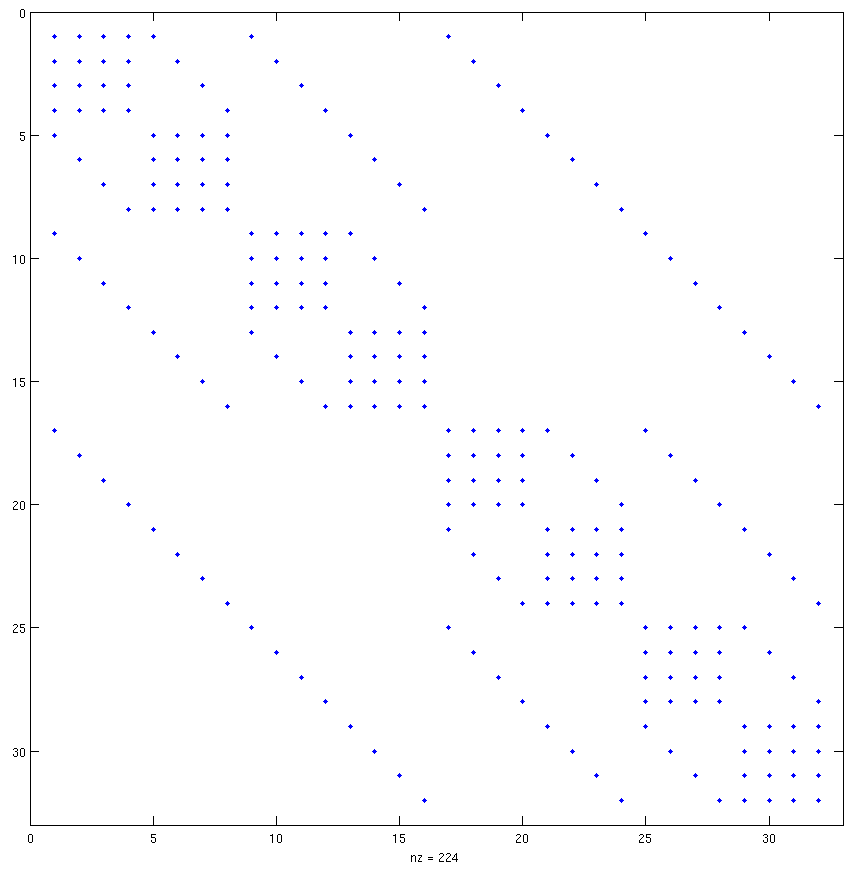
\includegraphics[width=3in]{chapters/spn_equations/group1.png}
  \end{center}
  \caption{\textbf{Sparsity pattern for 1-group $SP_7$
      discretization.} \textit{A $2\times 2 \times 2$ element mesh was
      used to show detail of the blocks formed by the discretization.}}
  \label{fig:group1}
\end{figure}
\begin{figure}[t!]
  \begin{center}
    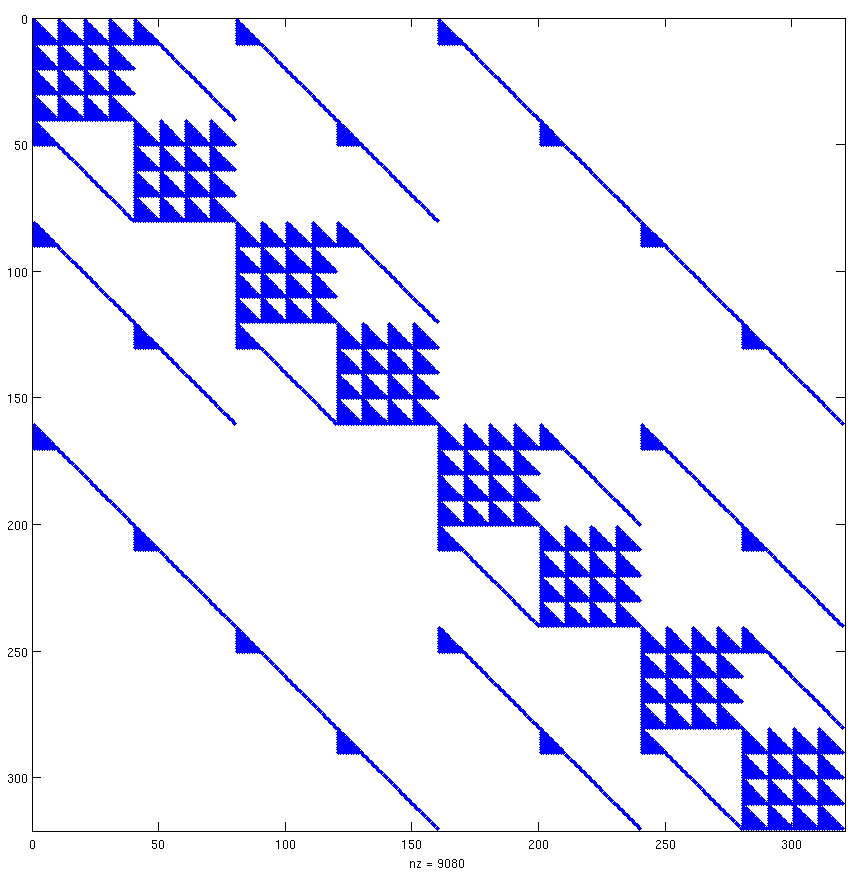
\includegraphics[width=3in]{chapters/spn_equations/group10ds.png}
  \end{center}
  \caption{\textbf{Sparsity pattern for 10-group $SP_7$ discretization
      with downscatter only.} \textit{A $2\times 2 \times 2$ element
      mesh was used to show detail of the blocks formed by the
      discretization.}}
  \label{fig:group10ds}
\end{figure}
\begin{figure}[t!]
  \begin{center}
    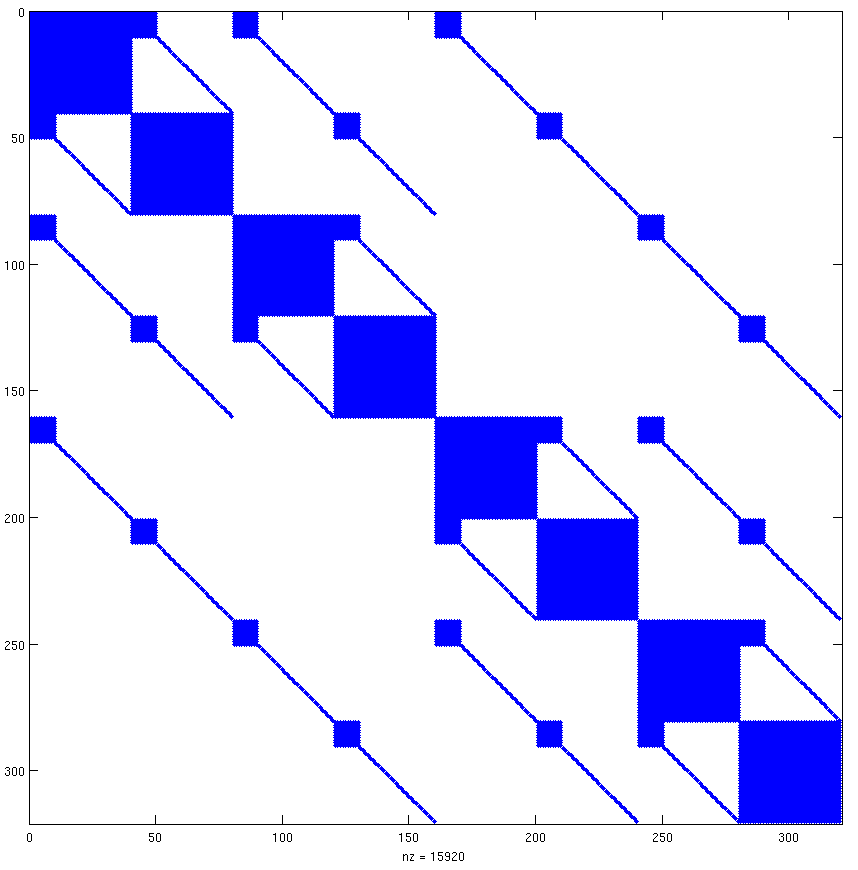
\includegraphics[width=3in]{chapters/spn_equations/group10us.png}
  \end{center}
  \caption{\textbf{Sparsity pattern for 10-group $SP_7$ discretization
      with downscatter and upscatter.} \textit{A $2\times 2 \times 2$ element
      mesh was used to show detail of the blocks formed by the
      discretization.}}
  \label{fig:group10us}
\end{figure}
We note a few key features of the sparsity plots. The first is that
for multigroup problems without full upscatter and downscatter
(i.e. Figure~\ref{fig:group10ds}), the resulting matrix is asymmetric
and therefore a linear solver that can handle asymmetric linear
systems is required. Nearly all problems of interest will not have
full upscattering or downscattering. Second we note the largely
diagonal character of these systems, although the blocks from
Eq~(\ref{eq:A_block_matrix}) are readily apparent. Our first attempt
at preconditioning this system will be to use the point Jacobi
preconditioning from \S\ref{sec:stochastic_preconditioning} due to
this diagonal form.

\subsection{Point Jacobi Spectral Analysis Results}
\label{subsec:spn_analysis_results}
Spectral radius computations were performed for the cases described
above for the point Jacobi preconditioned iteration matrix $\ve{H} =
\ve{I}-\ve{M}^{-1}\ve{A}$ with $\ve{M} =
diag(\ve{A})$. Table~\ref{tab:group1pj} gives the results for the
1-group case, Table~\ref{tab:group10dspj} for the 10-group case with
full downscatter only and Table~\ref{tab:group10uspj} for the 10-group
case with full downscatter and full upscatter.
\begin{table}[t!]
  \begin{center}
    \begin{tabular}{cccccc}\hline\hline
      \multicolumn{1}{c}{}& 
      \multicolumn{1}{c}{}& 
      \multicolumn{1}{c}{}& 
      \multicolumn{1}{c}{$SP_N$ Order}& 
      \multicolumn{1}{c}{}& 
      \multicolumn{1}{c}{} \\
       &   & \textbf{1} & \textbf{3} & \textbf{5} & \textbf{7}  \\
       & \textbf{0} & 0.0635 & 0.6722 & 1.3144 & 1.976 \\
       & \textbf{1} & 0.0666 & 0.6728 & 1.3141 & 1.9755 \\
      $P_N$ Order & \textbf{3} & 0.0666 & 0.6822 & 1.3141 & 1.9755 \\
       & \textbf{5} & 0.0666 & 0.6822 & 1.3278 & 1.9847 \\
       & \textbf{7} & 0.0666 & 0.6822 & 1.3278 & 1.9917 \\
      %%
      \hline\hline
    \end{tabular}
  \end{center}
  \caption{\textbf{Spectral radius results for the point Jacobi
      preconditioned iteration matrix with 1 energy group.}}
  \label{tab:group1pj}
\end{table}
\begin{table}[t!]
  \begin{center}
    \begin{tabular}{cccccc}\hline\hline
      \multicolumn{1}{c}{}& 
      \multicolumn{1}{c}{}& 
      \multicolumn{1}{c}{}& 
      \multicolumn{1}{c}{$SP_N$ Order}& 
      \multicolumn{1}{c}{}& 
      \multicolumn{1}{c}{} \\
       &   & \textbf{1} & \textbf{3} & \textbf{5} & \textbf{7}  \\
       & \textbf{0} & 0.0655 & 0.677 & 1.32 & 1.982 \\
       & \textbf{1} & 0.071 & 0.67777 & 1.319 & 1.982 \\
      $P_N$ Order & \textbf{3} & 0.071 & 0.687 & 1.327 & 1.9872 \\
       & \textbf{5} & 0.071 & 0.687 & 1.336 & 1.997 \\
       & \textbf{7} & 0.071 & 0.687 & 1.336 & 1.9995 \\
      %%
      \hline\hline
    \end{tabular}
  \end{center}
  \caption{\textbf{Spectral radius results for the point Jacobi
      preconditioned iteration matrix with 10 energy groups and full
      downscatter.}}
  \label{tab:group10dspj}
\end{table}
\begin{table}[t!]
  \begin{center}
    \begin{tabular}{cccccc}\hline\hline
      \multicolumn{1}{c}{}& 
      \multicolumn{1}{c}{}& 
      \multicolumn{1}{c}{}& 
      \multicolumn{1}{c}{$SP_N$ Order}& 
      \multicolumn{1}{c}{}& 
      \multicolumn{1}{c}{} \\
       &   & \textbf{1} & \textbf{3} & \textbf{5} & \textbf{7}  \\
       & \textbf{0} & 0.7283 & 0.81 & 1.47 & 2.1446 \\
       & \textbf{1} & 0.7317 & 0.8 & 1.46 & 2.1368 \\
      $P_N$ Order & \textbf{3} & 0.7317 & 0.91 & 1.526 & 2.2274 \\
       & \textbf{5} & 0.7317 & 0.91 & 1.5344 & 2.2562 \\
       & \textbf{7} & 0.7317 & 0.91 & 1.5345 & 1.2842 \\
      %%
      \hline\hline
    \end{tabular}
  \end{center}
  \caption{\textbf{Spectral radius results for the point Jacobi
      preconditioned iteration matrix with 10 energy groups, full
      downscatter and full upscatter.}}
  \label{tab:group10uspj}
\end{table}
It is readily apparent from the tabulated data the point Jacobi
preconditioning is insufficient as a preconditioning mechanism for
problems of order $SP_5$ or higher. In addition, as upscatter is
introduced into the system, a much larger spectral radius is observed
at lower $SP_N$ orders, signaling a need for a better preconditioning
strategy to both ensure and improve covergence for Monte Carlo
methods. 

\subsection{Preconditioning Strategy}
\label{subsec:spn_preconditioning}
If Monte Carlo methods are to be used to solve the $SP_N$ system of
equations, a different preconditioning strategy is required in order
to ensure convergence for systems of all $SP_N$ and $P_N$ orders with
arbitrary energy group structures. To achieve this, we look back to
the sparsity plots we generated in Figures~\ref{fig:group1},
\ref{fig:group10ds} and \ref{fig:group10us} as well as the multigroup
$SP_N$ equations. Initially, the diagonal character of the system led
us to try point Jacobi preconditioning with only marginal
results. From the sparsity plots we note the block structure that
ultimately arises from the multigroup scattering matrices and their
insertion into Eq~(\ref{eq:A_block_matrix}). When full upscatter and
downscatter are used the resulting blocks are completely dense while
only downscatter gives a lower triangular scattering matrix and the
block structure shown in Figure~\ref{fig:group10ds}. 

Based on this both block and diagonally dominant structure for
matrices formed by the general multigroup $SP_N$ equations, we instead
choose \textit{block Jacobi} preconditioning as a left preconditioner
for the system. Like point Jacobi preconditioning, block Jacobi
preconditioning extracts the diagonal elements of the matrix as the
preconditioner where now the elements extracted are the blocks on the
diagonal as shown on the left side of
Figure~\ref{fig:block_jacobi_ex}.
\begin{figure}[t!]
  \begin{center}
    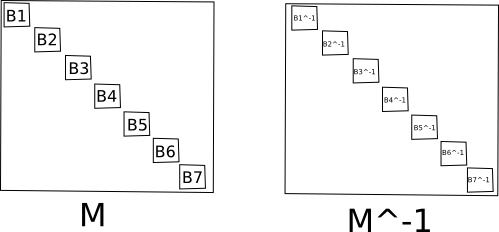
\includegraphics[width=5in]{chapters/spn_equations/block_preconditioning.png}
  \end{center}
  \caption{\textbf{Block Jacobi preconditioning strategy used for the
      $SP_N$ equations.} \textit{Left: The preconditioner is formed by
      the diagonal blocks of the matrix. Right: Inversion is trivial
      and decoupled by block.}}
  \label{fig:block_jacobi_ex}
\end{figure}
The inversion of this preconditioner is trivial as shown on the right
side of Figure~\ref{fig:block_jacobi_ex}. Each block can be inverted
individually and combined to form the inverse. For high performance
implementations this has several attractive properties. First, the
blocks in the matrix come from the energy/angle discretization of the
transport equation as given by Eq~(\ref{eq:A_block_matrix}). Each
block on the diagonal is bound to a mesh element in the system (note
there are 8 blocks on the diagonal in each of the sparsity patterns
with a mesh of $2 \times 2 \times 2$) and therefore we expect the
matrix elements forming the block to be entirely local. Second, these
blocks are typically dense and nearly lower triangular for many
transport problems meaning that established dense matrix methods based
on LU-factorization and other schemes can be used for fast inversion
\citep{lapack_citation}.

\subsection{Block Jacobi Spectral Analysis Results}
\label{subsec:spn_analysis_results}
